% Based on the answer by qubyte at 
% http://tex.stackexchange.com/questions/9767/whats-a-good-package-for-typesetting-quantum-circuits
\documentclass[12pt]{standalone}
\usepackage{tikz}

\usetikzlibrary{backgrounds}
% Dirac Kets
\newcommand{\ket}[1]{\ensuremath{\left|#1\right\rangle}}

\begin{document}
    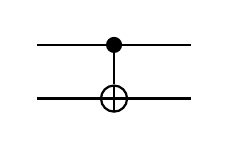
\begin{tikzpicture}[thick,cross/.style={path picture={ 
  \draw[black]
(path picture bounding box.south) -- (path picture bounding box.north);
}}]

    % `operator' will only be used by most gates.
    % `cnot' will refer to CNOT gates.
    % `phase' is used for controlled gates.
    \tikzstyle{operator} = [draw,fill=white,minimum size=1.5em]
    \tikzstyle{cnot} = [draw,cross,circle,minimum size=5pt]
    \tikzstyle{phase} = [draw,fill,shape=circle,minimum size=5pt,inner sep=0pt]
    %
    \matrix[row sep=0.4cm, column sep=0.8cm] (circuit) {

    % First row.
    \coordinate (start1); &
    \node[phase] (P11) {}; &
    \coordinate (end1);\\

    \coordinate (start2); &
    \node[cnot] (O21) {}; &
    \coordinate (end2);\\
    };

    \begin{pgfonlayer}{background}
        % Draw lines.
        \draw[thick] (start1) -- (end1) (start2) -- (end2) (P11) -- (O21);
    \end{pgfonlayer}
    %
    \end{tikzpicture}
\end{document}
